\section{Batch Layer}

The batch layer is the heart of the Lambda architecture.
It is the place where all ever gathered data resides and being processed.
The batch layer executes two main tasks: storing of data arriving from outer sources, and processing of that data to create batch views, used for the low-latency query answering.
The first issue requires usage of a storage system that provides fast appending, efficient batch reads, and no random reads/writes of data.
Computation of batch views demands application of distributed efficient batch processing algorithms as for example MapReduce.

\subsection{Data Model}

The batch layer requires usage of a specific data model to make the Lambda architecture scalable, highly efficient and fault-tolerant.
This data model is based upon four main notions.
\textit{Information} - the whole knowledge, that system holds.
\textit{Data} - collecting notion for records, strings, values, etc., kept in the system, so that they cannot be derived from any other data.
\textit{Query} - a question that is asked to the system, and demands a piece of information that answers it.
\textit{View} - a data structure that holds information directly useful for answering query.

\mnote{Raw data}
To answer as much different queries as possible, the batch layer stores only \textit{raw data}.
It is possible to derive from it data, particularly relevant for query, but not vice versa.
This is important, because the system does not know in advance all queries it will have to answer in the feature.
The more basic is the data, the more information can be possibly deduced from it.

In the current context, unstructured data is always better than normalized, because it is rawer.
As an example, let us consider the system, that stores users' search of a geographic location.
Suppose that system stores all those queries for further analytics.
If it saves them normalized, or in other words parsed and mapped to a known geographic location, it can for certain queries save nothing or NULL value, because algorithm cannot execute correct mapping.
In other case, when the system stores raw string, that user typed, it can later on have this data properly parsed, if parsing and mapping algorithms are improved.
This example shows, that unstructured raw data is preferred to store in the batch layer.

\mnote{Data immutability}
The batch layer does not allow modification or deletion of data, what is called \textit{immutability}.
It only allows appending new records.
This property gives two crucial advantages.
Immutability dramatically simplifies complexity of the storage mechanisms.
This is because maintenance of modifications in the distributed environment is not an easy task.
To successfully update a record, the system must perform it for all replications, provide locks and prohibit simultaneous updates.
It has to maintain versions of the same record for different users.
Absence of all these and many other requirements saves from much of complexity.
The system is easier to understand, repair and improve.
It is much safer from programming mistakes and consequent errors.

\mnote{Human fault-tolerance}
Another advantage of immutability is that mistakes in algorithms cannot corrupt data anymore.
This property is called \textit{human fault-tolerance}, and it is very important, because programmers always do mistakes.
As a result, it is possible, that wrong code can incorrectly update or delete data.
When data is immutable, programmers' mistakes can only append wrong data to the dataset.
This can be later repaired by administrator, but all proper data is always safe.

Immutability leads to high growth of data volume, because everything last stored basically forever.
This is, however, not a problem, because, as we discuss later on in this chapter, the batch layer is purely distributed and scalable.
It allows increasing capacity of its data store to any extent, adding new machines at any time.

Immutability requires completely different data model, comparing to relational databases, that manipulate tuples of complex objects altogether.
In contrast, the batch layer stores each attribute of a logical tuple separately.
Each value has the timestamp of addition moment. 
Such technique allows having the whole history of logical updates of all records.
The actual value is the one with the oldest timestamp.

\mnote{Eternal truthfulness of data}
Immutability gives one more important property of data, stored in the batch layer, namely \textit{eternal truthfulness of data}.
When new record is added, no matter is it a new piece of data or update of an old data, it represents true information in that particular moment in time.
This never becomes false, because it describes event or state of the world that is an occurred fact.
This property implies that the batch layer not only stores data, describing the state of the system, but also the history of its state changes.

\mnote{Master dataset}
Having defined the main properties of data, we can introduce the notion of the \textit{master dataset}.
The master dataset is the main storage, where all the data that ever arrived to the system resides.
The batch layer is responsible for its maintenance.
If there is a fault of the master dataset - all data can be lost.
And data is of the most importance in this context.
Therefore, the master dataset must be carefully designed, set up and protected.
It must be saved from all types of failures, e.g. software, hardware or human.
The master dataset is logically a large list of records.
When new piece of data arrives into the system, the batch layer appends it to the master dataset.
The more exact description of how the master dataset can look like will be discussed later on in this chapter.

\begin{table}[h]
  \centering
  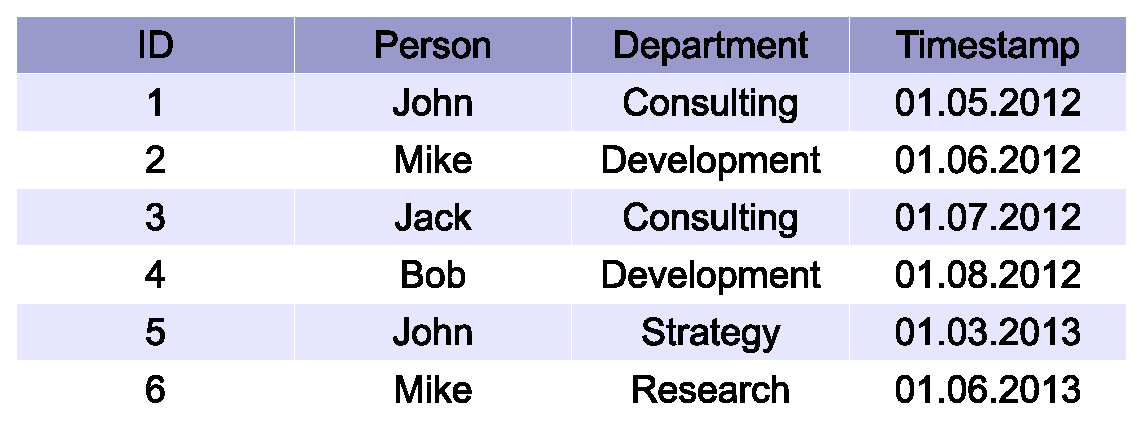
\includegraphics [width=0.8\textwidth]{images/MasterDatasetExample}
  \caption{An example of the list of records in the master dataset.}
  \label{tab:MasterDatasetExample}
\end{table}

On the Table~\ref{tab:MasterDatasetExample} there is an example of the list of records of the master dataset.
The 5th and 6th records are updates of the 1st and 2nd, respectively.
They are in the same list, but the current version is defined by the last timestamp.
This model implies, that the whole history of updates is available at any time in the future. 

\mnote{Fact-based model}
In contrast to relational databases, data in the master dataset is stored using a so called \textit{fact-based model}.
It supposes that all the data is divided into simple units called facts.
Fact has several properties.
It is timestamped on addition to the master dataset.
Fact cannot be divided to a smaller units, it is already atomic.
Fact is identifiable in the sense that any two facts in the dataset must be distinguishable.

Fact-based model offers several important advantages.
It allows to make queries to a state of the dataset at any time in its history, because each piece of data (fact) is timestamped and immutable, or, in other words, eternally true.
It provides human-fault tolerance, as long as facts are immutable, and if a fact is added mistakenly, administrator can delete it.
If any of attributes of a complex object are absent, it is not necessary to store any NULL values, because data is stored in atomic facts.
Data can be stored in an unstructured denormalized form, because it is not queried directly from the master dataset, but from batch views of the serving layer, discussed later on.

\mnote{Graph schema}
To unite facts into related data there are so called \textit{graph schemas}.
Graph schema is a graph that describes the structure of a fact-based model.
It defines relations between entities similarly as entity-relationship model does for relational databases.
Graph schema consists of three elements: nodes, edges and properties.
Nodes are entities representing particular objects of a describable system.
Edges define relationships that connect nodes into the specific structure.
Properties provide information associated with nodes.

\begin{figure}[h]
  \centering
  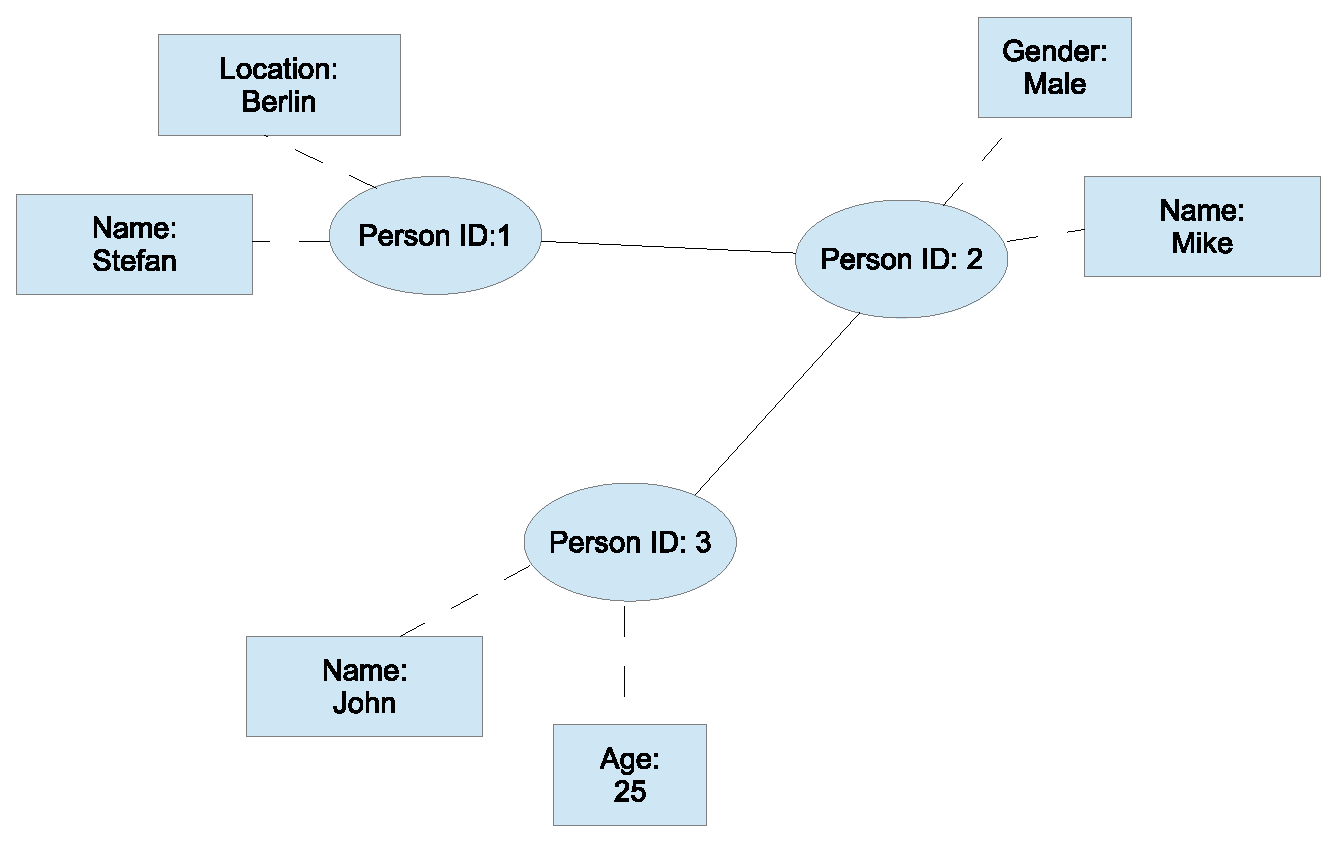
\includegraphics [width=0.8\textwidth]{images/GraphSchema}
  \caption{An example of graph schema.}
  \label{fig:GraphSchema}
\end{figure}

Figure~\ref{fig:GraphSchema} shows an example of a graph schema for a simple data model.
Entities are represented using ovals.
They are persons in this case.
Users are connected with their properties via dashed lines.
Lines between entities are edges.

\mnote{Serialization frameworks}
To save developers from detailed implementation of graph schema every time, and from possibility to do mistakes during this process, there are so called \textit{serialization frameworks}.
They provide a useful tool that generates all needed code, having described schema of the dataset in a specific descriptive language.
Serialization frameworks require only description of key notions, e.g. nodes, edges and properties.
They enforce then generation of all additional data fields and proper structure and data types for defined elements, as for example timestamps.  
Examples of serialization frameworks are Avro \ref{subs:avro} and Thrift \ref{subs:thrift}.

\subsection{Data Storage}

Physical data storage of the master dataset is another important issue.
In the big data context it is not possible to store all the data on one server.
Hence, distributed solution, that provides easy access, scalability and fault-tolerance, is required. 

\mnote{Requirements}
To understand requirements to the data storage, it is important to understand how data is going to be written and read.
Two main actions, it must support, are appending of new records and a bulk read for batch processing.
Immutability of data and continual appending demand, that high growth of the size of the master dataset must be easily affordable and maintainable.
Bulk reads require ability to access data in a parallel fashion.
There is no need for random writes or reads, what simplifies things dramatically.
Another important issue that the master dataset must allow to access only useful (for particular computations) parts of data.
This property is called \textit{vertical partitioning}.
The last requirement is that the master dataset must provide flexible way to store data compressed.

\mnote{Usage of HDFS}
There are many solutions that fulfil all described properties, starting from distributed file systems and finishing with distributed database systems. 
We choose the \textit{Hadoop Distributed File System} (HDFS), that we describe later on in all details \ref{subs:HDFS}.
Briefly, its main properties are: complete distributiveness that allows addition of as many new nodes as required, fault-tolerance via replication of data, high throughput via parallel access, tight connection with Hadoop MapReduce, simple access to the tree-structured file data.
HDFS fulfils all requirements that were stated for the master dataset storage system.

As long as HDFS stores data in the tree of files and folders, the way of applying it for the master dataset is straightforward.
All the data of the master dataset is then stored in the common folder.
Each piece of data, containing possible a set of records, is stored in a separate file that is automatically replicated.
There is also a necessity to fuse several small files into one big file periodically to avoid fragmentation and to increase batch access throughput.

An example of abstraction of the access to files and directories, that can be used to simplify access to HDFS, and to avoid use of a low-level HDFS API, is a \textit{Pail}.
Pail is a Java library, that allows working with HDFS in a more object-oriented way.
It makes code shorter an easier to read, and saves from many standard mistakes, that occur working with HDFS directly.

\subsection{Computation of Batch Views}

Answering particular query is often unreasonably expensive or even infeasible in the real time.
This is because amount of available data is huge, and because this data is raw. 
Moreover, query answer demands usually a piece of information that is far away from what raw data describes.
It requires often execution of complex algorithms on the whole dataset.
In the BigData context that can mean hours of processing, while low-latency response is typically a condition.

To solve this issue the batch layer precomputes batch views in advance.
Batch views contain derived data that is a result of execution of specific algorithms and aggregations on the whole dataset.
They help in answering particular queries.
The batch layer creates batch views in advance, so that they are ready for low-latency response in the query time.

The batch layer computes batch views in the infinite loop.
After completion of data processing, it starts from the beginning.
Processing of all the data and creating batch views is a long operation.
It can take hours and even days to be done.
As a result batch views are always out-of-date.
This is, however, can be considered as a deep analysis of data that connect pieces together to produce intelligent inference.
To overcome an issue of a long time processing, the Lambda architecture introduces the speed layer that we discuss in details later on in this chapter.

The batch layer executes specific functions on the master dataset that result in batch views.
These batch views store data that is easy to use to answer particular queries on the fly.
But it is important to mention, that this is not exact values that satisfy clients queries.
Rather, batch views hold data that can be on the fly used by the serving layer.
Storing of endpoint values would be in many cases way too expensive or even infeasible.
%Figure~ [add figure] shows this approach.

\mnote{Recomputation and incremental algorithms}
There are two approaches to compute batch views: to recompute them from scratch, and to make incremental updates.
Both of them have advantages and disadvantages that are the consequence of three properties: performance, human fault-tolerance, and generality of the algorithm.
Performance is usually much higher for incremental algorithms to compute batch views, because they simple do not have to process the whole master dataset, but only new data after previous processing.
But batch views has to be designed in a more complex way to allow incremental updates, what makes them usually larger, and slower to update.
Human fault-tolerance is inherent for the recomputational model.
If there is a mistake in building of batch views, it requires only removing that bug and deploying new code.
After next batch processing batch views will be properly created.
In contrast, for incremental method, it can be hard to find and correct results of mistakes in the algorithm.
It requires repairing of batch views, what is not an easy task in many cases.
Generality of the algorithm is a standard property of recomputational model.
Computations are simple and easy to tune, if query needs are changed.
Incremental algorithms are often approximated, what leads to a possible with some probability error in answering query.
They also move usually the part of computations to the querying time, what makes latency of the system's response higher.
As a result, it is strongly recommended to use recomputational algorithms.

\mnote{Application of Hadoop MapReduce}
Computation of batch views is an inherently distributed operation.
Developer does not have to think about multithreading issues.
He only writes simple one-threaded code, that is distributed then automatically in the cluster.
MapReduce is a perfect example of batch processing.
We have already discussed MapReduce programming paradigm in details in the Section~\ref{sec:mapreduce}.
Framework Apache Hadoop, based on HDFS, provides a powerful implementation of the MapReduce.
It is available for free as an open source product, and requires from developer only an implementation of \lstinline{map} and \lstinline{reduce} functions, what makes batch processing easy to implement in the real system.